\chapter{Logic internal representation}

When talking about formula we would often describe formula by $n$ number of elements, eg. formula has 4 predicates. In sense of implementation more specyfic vocabulary is needed. From now on when talking abount $n$ occurrences of element, mathematical sense is assumed (usually it is element name and arity). In implementation user will be asked to provide \textit{signature} of element. Signature is differentiated by argument types that is holds. This is importatant thus name of signature is often irrelevant and can be filled later. Element \textit{instance} is every occurance of in formula.

\begin{table}
  \centering
  \small
  \begin{tabularx}{\textwidth}{|c|X|X|}
    \hline
    FOL element & Mathematical sense & Signature \\
    \hline
    Variable & by name and scope? $V1$, $V2$ & there is only one signature for variable \\  
    \hline
    Functor & by name and arity $f/0$, $f/1$ & by types of arguments $f(Variable)$, $f(functor)$ \\
    \hline
    Predicate & by name and arity $p/0$, $p/1$ & by types of arguments $p(Variable)$, $p(functor)$ \\
    \hline
    Atom & by connective and operands $p/0$, $p/1 = V$ & by connective and operands signatures $p(Variable)$, $p(Variable) = p(Functor)$ \\
    \hline
    Literal & by negation sign and atom & by negation sign and atom signature \\
    \hline
    Clause & by ? & \\
    \hline
    Formula & & \\
    \hline
  \end{tabularx}
  \caption{Comparison of how elements of FOL in sense of math and signature}
\end{table}


In this chapter every element of \gls{FOL} will be described in context of implementation along with some computational complexity adnotations.

\section{First Order Logic elements}

\begin{figure}[H]
\begin{centering}
  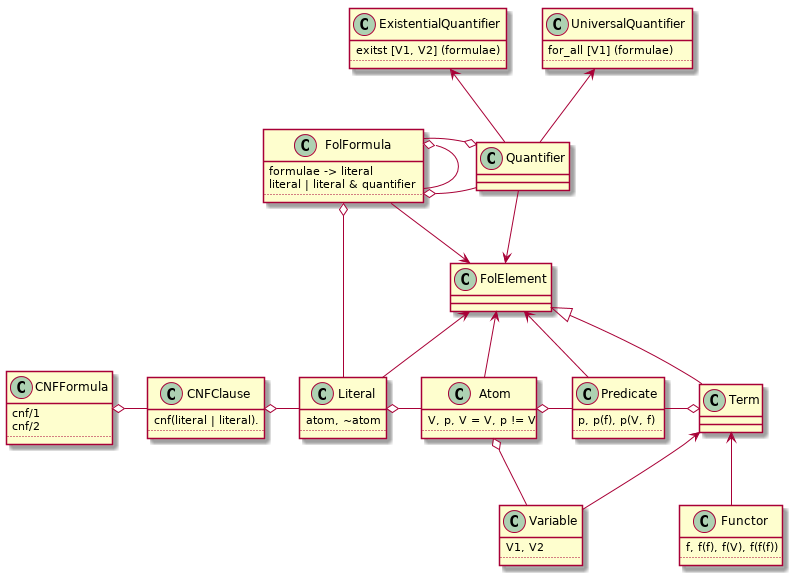
\includegraphics[width=\textwidth]{logic-formula-generator/fol/fol_elements.png}
  \caption{Class diagram for FOL}
\end{centering}
\end{figure}

\subsection{Functor}

Functor can contain variable or another functor.
Given that
$n$ is functor recursion depth,
$a$ is functor arity,
we can produce $f(n, a)$ number of functor signatures

\begin{align*}
	&f(n, a) =
	\begin{cases}
		a, \text{for } n = 0, \\
		a \sum_{i=n}^{i=1} \sum_{j=a}^{j=0} f(n-i,a-j) \\
	\end{cases} \\
\end{align*}

\subsection{Predicates}

Predicates can contain functors or variables.

How many types (ignoring predicate, functor and variable name) of predicates $P$ can be produced, knowing that:
\begin{itemize}
	\item functor arity $a_f$ is in range $[a_{f1}, a_{f2}]$,
	\item functor recursion depth $n$ is less or equal to $n_{max}$,
	\item $a_p$ is predicate arity?
\end{itemize}

\begin{align*}
	f_t(n_{max}, a_{fmin}, a_{fmax}) &= \sum_{i=0}^{n_{max}} \sum_{j=a_{f1}}^{a_{f2}} f(i, j), \\
	P(a_p) &=
	\begin{cases}
		1, \text{for } a_p = 0 \\
		(f_t(n_{max}, a_{fmin}, a_{fmax}) + 1)^{a_p}, \\
	\end{cases} \\
	\text{where} \\
	f_t(n_{max}, a_{fmin}, a_{fmax}) & \text{ -- total number of functors} \\
\end{align*}

\subsection{Atoms}

Atom can contain variabe or predicate. Atom connects items with binary mathematical connective: $=$ or $!=$.

How many types of atoms $A$ can be produced, knowing that:
\begin{itemize}
	\item predicate arity $a_p$ is given as set of $\{1,2,\dots\}$?
\end{itemize}

\begin{align*}
	A(a_p) &=
	\text{where} \\
	& \text{ -- total number of functors} \\
\end{align*}

\subsection{Literals}

\subsection{CNF Clause}

Clause $C$ can contain only literals. The order of literals is not important.

\begin{align*}
	&C = \{l1, 12, \dots\}
\end{align*}

How many different clauses can be produced, knowing that:
\begin{itemize}
	\item clause length is $x$
	\item given set of literals $L = \{l1, l2, \dots\}$, $\forall_{i,j \in L} i \neq j$
\end{itemize}

\begin{align*}
	&C(x) = \binom{|L|}{x}, \\
	\text{where }
	&|L| \text{ -- number of elements in L} \\
\end{align*}

\subsection{CNF formulas}

How many different cnf formulas can be produced, knowing that:
\begin{itemize}
	\item formula contains $x$ clauses
	\item given set of clauses $C = \{c1, c2, \dots\}$, $\forall_{i,j \in L} i \neq j$
\end{itemize}

\begin{align*}
	&F_{cnf}(x) = \binom{|C|}{x}, \\
	\text{where }
	&|C| \text{ -- number of elements in C} \\
\end{align*}

\section{CNF Generator parameters}

User defines generator in 3 steps.
\begin{enumerate}
  \item \textbf{Allowed FOL signatures}

    In this step user defines set of allowed \gls{FOL} elements:
    \begin{itemize}
      \item set of allowed functor arities $a_f = \{0, 1, 2,\dots\}$
      \item maximum recursion depth $n$ for functors
      \item set of allowed predicate arities $a_p = \{0, 1, 2,\dots\}$
      \item set of atom allowed connectives, that is no connective or/and any subset of $AllowedConnectives = \{=, !=\}$
      \item if negated literals are allowed
      \item set of allowed clause lengths $AllowedClausesLen = \{1,2,\dots\}$
      \item set of allowed number of clauses in formula $AllowedFormulaLen = \{1,2,\dots\}$
    \end{itemize}
  \item \textbf{How many instances of elements are allowed}

    In this step user defines what properties formula should have:
    \begin{itemize}
      \item formula contains from $c_{min}$ to $c_{max}$ clauses, but the best solution is considered middle of this range
      \item formula contains from $l_{min}$ to $l_{max}$ literals, but the best solution is considered middle of this range
      \item TODO more params
    \end{itemize}
  \item \textbf{Names for term-like FOL elemnents}

    In this step user defines:
    \begin{itemize}
      \item set of variable names $\{'v1','v2',\dots\}$
      \item set of functor names $\{'f1','f2',\dots\}$
      \item set of predicate names $\{'p1','p2',\dots\}$
    \end{itemize}
\end{enumerate}
